% ============================================================================
%  fig_ablation_waterfall.tex  --  additive-ablation waterfall on AP50 (TikZ).
%  Colours match the draw.io / Gemini version exactly (HEX below).
%  Needs \usepackage{tikz} in the preamble (added to thesisstyle.sty).
%  Include with:  % ============================================================================
%  fig_ablation_waterfall.tex  --  additive-ablation waterfall on AP50 (TikZ).
%  Colours match the draw.io / Gemini version exactly (HEX below).
%  Needs \usepackage{tikz} in the preamble (added to thesisstyle.sty).
%  Include with:  % ============================================================================
%  fig_ablation_waterfall.tex  --  additive-ablation waterfall on AP50 (TikZ).
%  Colours match the draw.io / Gemini version exactly (HEX below).
%  Needs \usepackage{tikz} in the preamble (added to thesisstyle.sty).
%  Include with:  % ============================================================================
%  fig_ablation_waterfall.tex  --  additive-ablation waterfall on AP50 (TikZ).
%  Colours match the draw.io / Gemini version exactly (HEX below).
%  Needs \usepackage{tikz} in the preamble (added to thesisstyle.sty).
%  Include with:  \input{tikz/fig_ablation_waterfall}
%  y = (AP50 - 0.838) * 333.333 cm  (axis zoomed to 0.838-0.856)
% ============================================================================
\definecolor{wfBaseFill}{HTML}{DAE8FC}
\definecolor{wfBaseStroke}{HTML}{6C8EBF}
\definecolor{wfGainFill}{HTML}{D5E8D4}
\definecolor{wfGainStroke}{HTML}{82B366}
\definecolor{wfRedEdge}{HTML}{FF0000}
\definecolor{wfMambaFill}{HTML}{F8CECC}
\definecolor{wfMambaStroke}{HTML}{B85450}
\definecolor{wfGreenText}{HTML}{2D7D2D}
\definecolor{wfRedText}{HTML}{C00000}
\definecolor{wfGrey}{HTML}{999999}
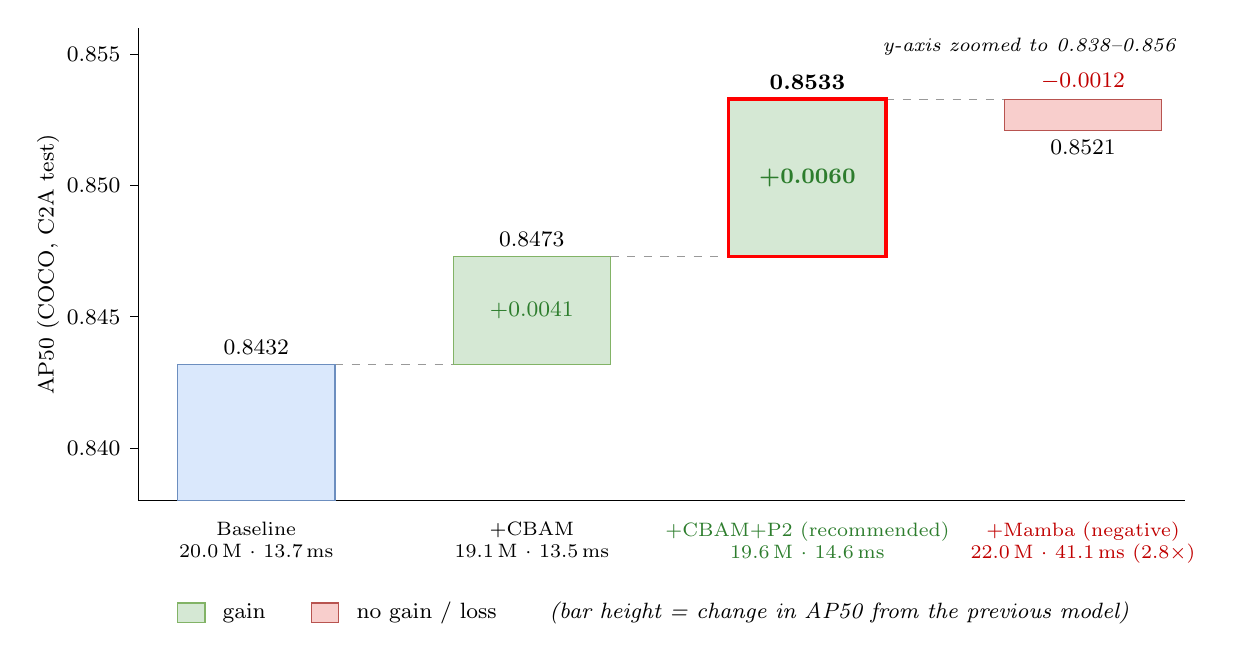
\begin{tikzpicture}[font=\footnotesize]
  % ---- axes ----
  \draw[black] (1.0,0) -- (1.0,6.0);
  \draw[black] (1.0,0) -- (14.3,0);
  \foreach \y/\lab in {0.6667/0.840, 2.3333/0.845, 4.0/0.850, 5.6667/0.855}{%
    \draw[black] (0.9,\y) -- (1.0,\y);
    \node[left] at (0.9,\y) {\lab};
  }
  \node[rotate=90,anchor=south] at (0.12,3.0) {AP50 (COCO, C2A test)};
  \node[anchor=north east,font=\itshape\scriptsize] at (14.3,6.0) {y-axis zoomed to 0.838--0.856};

  % ---- dashed step connectors ----
  \draw[wfGrey,dashed] (3.5,1.7333) -- (5.0,1.7333);
  \draw[wfGrey,dashed] (7.0,3.1)    -- (8.5,3.1);
  \draw[wfGrey,dashed] (10.5,5.1)   -- (12.0,5.1);

  % ---- bars ----
  \filldraw[fill=wfBaseFill,draw=wfBaseStroke]                     (1.5,0)      rectangle (3.5,1.7333);
  \filldraw[fill=wfGainFill,draw=wfGainStroke]                     (5.0,1.7333) rectangle (7.0,3.1);
  \filldraw[fill=wfGainFill,draw=wfRedEdge,line width=1.2pt]       (8.5,3.1)    rectangle (10.5,5.1);
  \filldraw[fill=wfMambaFill,draw=wfMambaStroke]                   (12.0,4.7)   rectangle (14.0,5.1);

  % ---- resulting AP50 above/below each bar ----
  \node[above] at (2.5,1.7333) {0.8432};
  \node[above] at (6.0,3.1)    {0.8473};
  \node[above,font=\footnotesize\bfseries] at (9.5,5.1) {0.8533};
  \node[below] at (13.0,4.7)   {0.8521};

  % ---- per-step delta ----
  \node[text=wfGreenText]                       at (6.0,2.4167) {+0.0041};
  \node[text=wfGreenText,font=\footnotesize\bfseries] at (9.5,4.1) {+0.0060};
  \node[above,text=wfRedText]                   at (13.0,5.1)   {$-0.0012$};

  % ---- x-axis labels: model, params, latency ----
  \node[below,align=center,font=\scriptsize] at (2.5,-0.15)
        {Baseline\\20.0\,M $\cdot$ 13.7\,ms};
  \node[below,align=center,font=\scriptsize] at (6.0,-0.15)
        {+CBAM\\19.1\,M $\cdot$ 13.5\,ms};
  \node[below,align=center,font=\scriptsize,text=wfGreenText] at (9.5,-0.15)
        {+CBAM+P2 (recommended)\\19.6\,M $\cdot$ 14.6\,ms};
  \node[below,align=center,font=\scriptsize,text=wfRedText] at (13.0,-0.15)
        {+Mamba (negative)\\22.0\,M $\cdot$ 41.1\,ms (2.8$\times$)};

  % ---- legend ----
  \filldraw[fill=wfGainFill,draw=wfGainStroke]  (1.5,-1.55) rectangle (1.85,-1.30);
  \node[anchor=west] at (1.95,-1.425) {gain};
  \filldraw[fill=wfMambaFill,draw=wfMambaStroke] (3.2,-1.55) rectangle (3.55,-1.30);
  \node[anchor=west] at (3.65,-1.425) {no gain / loss};
  \node[anchor=west,font=\footnotesize\itshape] at (6.1,-1.425) {(bar height = change in AP50 from the previous model)};
\end{tikzpicture}

%  y = (AP50 - 0.838) * 333.333 cm  (axis zoomed to 0.838-0.856)
% ============================================================================
\definecolor{wfBaseFill}{HTML}{DAE8FC}
\definecolor{wfBaseStroke}{HTML}{6C8EBF}
\definecolor{wfGainFill}{HTML}{D5E8D4}
\definecolor{wfGainStroke}{HTML}{82B366}
\definecolor{wfRedEdge}{HTML}{FF0000}
\definecolor{wfMambaFill}{HTML}{F8CECC}
\definecolor{wfMambaStroke}{HTML}{B85450}
\definecolor{wfGreenText}{HTML}{2D7D2D}
\definecolor{wfRedText}{HTML}{C00000}
\definecolor{wfGrey}{HTML}{999999}
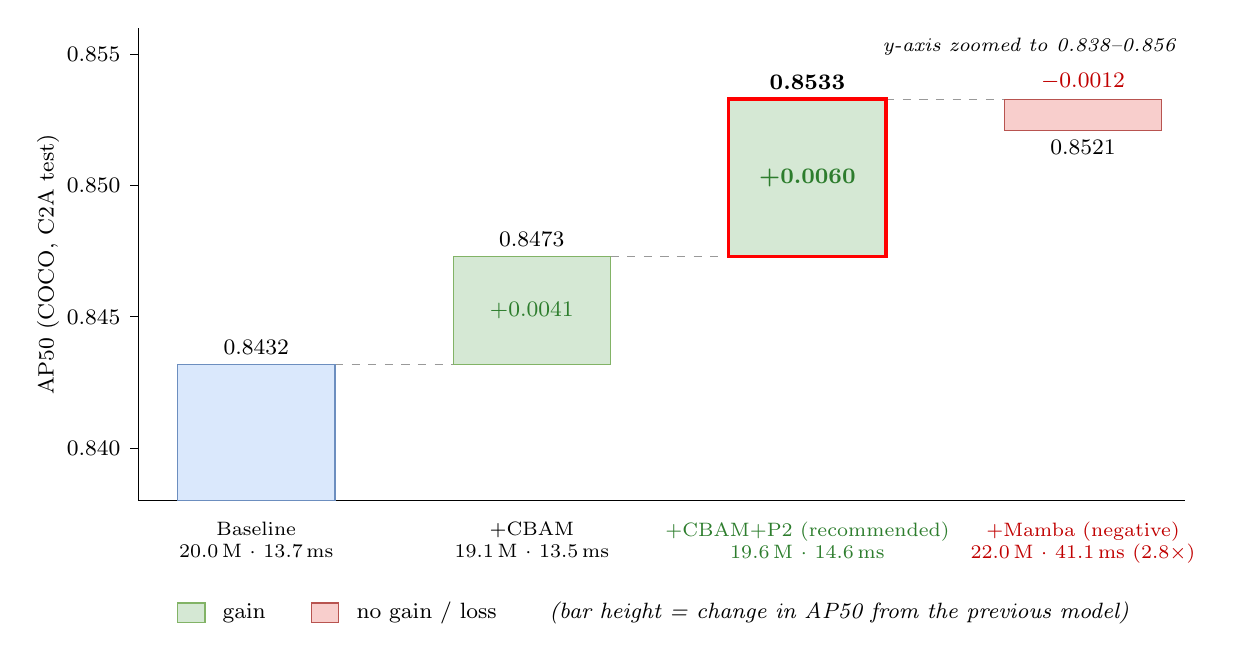
\begin{tikzpicture}[font=\footnotesize]
  % ---- axes ----
  \draw[black] (1.0,0) -- (1.0,6.0);
  \draw[black] (1.0,0) -- (14.3,0);
  \foreach \y/\lab in {0.6667/0.840, 2.3333/0.845, 4.0/0.850, 5.6667/0.855}{%
    \draw[black] (0.9,\y) -- (1.0,\y);
    \node[left] at (0.9,\y) {\lab};
  }
  \node[rotate=90,anchor=south] at (0.12,3.0) {AP50 (COCO, C2A test)};
  \node[anchor=north east,font=\itshape\scriptsize] at (14.3,6.0) {y-axis zoomed to 0.838--0.856};

  % ---- dashed step connectors ----
  \draw[wfGrey,dashed] (3.5,1.7333) -- (5.0,1.7333);
  \draw[wfGrey,dashed] (7.0,3.1)    -- (8.5,3.1);
  \draw[wfGrey,dashed] (10.5,5.1)   -- (12.0,5.1);

  % ---- bars ----
  \filldraw[fill=wfBaseFill,draw=wfBaseStroke]                     (1.5,0)      rectangle (3.5,1.7333);
  \filldraw[fill=wfGainFill,draw=wfGainStroke]                     (5.0,1.7333) rectangle (7.0,3.1);
  \filldraw[fill=wfGainFill,draw=wfRedEdge,line width=1.2pt]       (8.5,3.1)    rectangle (10.5,5.1);
  \filldraw[fill=wfMambaFill,draw=wfMambaStroke]                   (12.0,4.7)   rectangle (14.0,5.1);

  % ---- resulting AP50 above/below each bar ----
  \node[above] at (2.5,1.7333) {0.8432};
  \node[above] at (6.0,3.1)    {0.8473};
  \node[above,font=\footnotesize\bfseries] at (9.5,5.1) {0.8533};
  \node[below] at (13.0,4.7)   {0.8521};

  % ---- per-step delta ----
  \node[text=wfGreenText]                       at (6.0,2.4167) {+0.0041};
  \node[text=wfGreenText,font=\footnotesize\bfseries] at (9.5,4.1) {+0.0060};
  \node[above,text=wfRedText]                   at (13.0,5.1)   {$-0.0012$};

  % ---- x-axis labels: model, params, latency ----
  \node[below,align=center,font=\scriptsize] at (2.5,-0.15)
        {Baseline\\20.0\,M $\cdot$ 13.7\,ms};
  \node[below,align=center,font=\scriptsize] at (6.0,-0.15)
        {+CBAM\\19.1\,M $\cdot$ 13.5\,ms};
  \node[below,align=center,font=\scriptsize,text=wfGreenText] at (9.5,-0.15)
        {+CBAM+P2 (recommended)\\19.6\,M $\cdot$ 14.6\,ms};
  \node[below,align=center,font=\scriptsize,text=wfRedText] at (13.0,-0.15)
        {+Mamba (negative)\\22.0\,M $\cdot$ 41.1\,ms (2.8$\times$)};

  % ---- legend ----
  \filldraw[fill=wfGainFill,draw=wfGainStroke]  (1.5,-1.55) rectangle (1.85,-1.30);
  \node[anchor=west] at (1.95,-1.425) {gain};
  \filldraw[fill=wfMambaFill,draw=wfMambaStroke] (3.2,-1.55) rectangle (3.55,-1.30);
  \node[anchor=west] at (3.65,-1.425) {no gain / loss};
  \node[anchor=west,font=\footnotesize\itshape] at (6.1,-1.425) {(bar height = change in AP50 from the previous model)};
\end{tikzpicture}

%  y = (AP50 - 0.838) * 333.333 cm  (axis zoomed to 0.838-0.856)
% ============================================================================
\definecolor{wfBaseFill}{HTML}{DAE8FC}
\definecolor{wfBaseStroke}{HTML}{6C8EBF}
\definecolor{wfGainFill}{HTML}{D5E8D4}
\definecolor{wfGainStroke}{HTML}{82B366}
\definecolor{wfRedEdge}{HTML}{FF0000}
\definecolor{wfMambaFill}{HTML}{F8CECC}
\definecolor{wfMambaStroke}{HTML}{B85450}
\definecolor{wfGreenText}{HTML}{2D7D2D}
\definecolor{wfRedText}{HTML}{C00000}
\definecolor{wfGrey}{HTML}{999999}
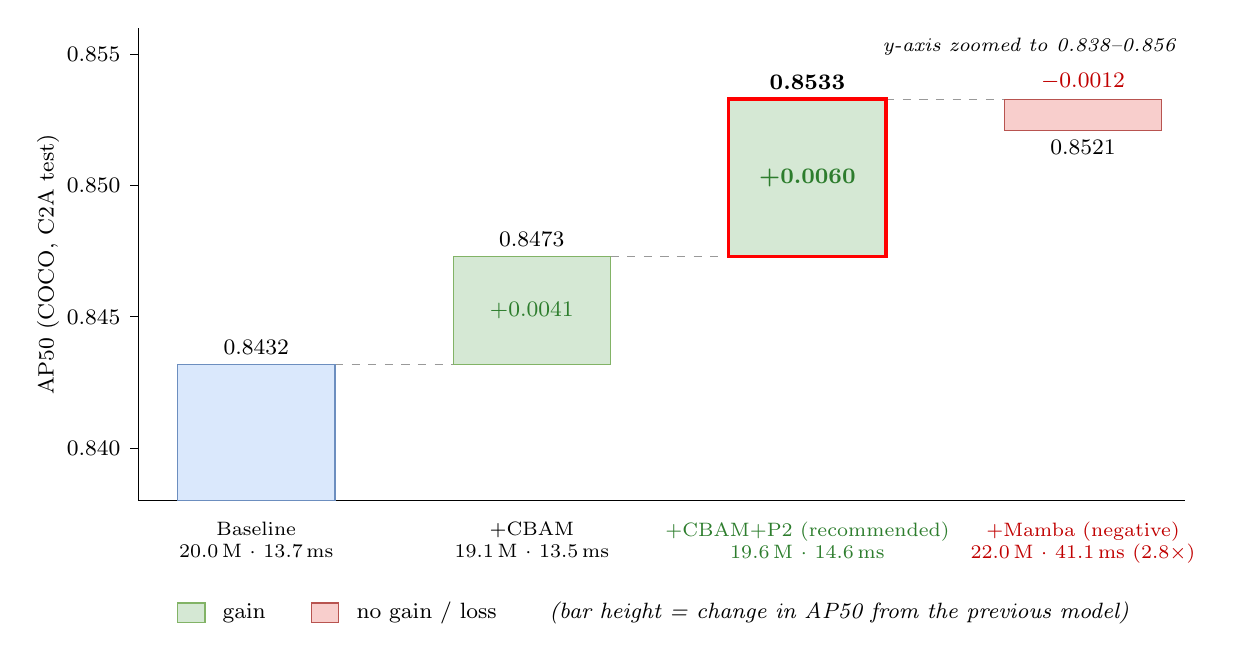
\begin{tikzpicture}[font=\footnotesize]
  % ---- axes ----
  \draw[black] (1.0,0) -- (1.0,6.0);
  \draw[black] (1.0,0) -- (14.3,0);
  \foreach \y/\lab in {0.6667/0.840, 2.3333/0.845, 4.0/0.850, 5.6667/0.855}{%
    \draw[black] (0.9,\y) -- (1.0,\y);
    \node[left] at (0.9,\y) {\lab};
  }
  \node[rotate=90,anchor=south] at (0.12,3.0) {AP50 (COCO, C2A test)};
  \node[anchor=north east,font=\itshape\scriptsize] at (14.3,6.0) {y-axis zoomed to 0.838--0.856};

  % ---- dashed step connectors ----
  \draw[wfGrey,dashed] (3.5,1.7333) -- (5.0,1.7333);
  \draw[wfGrey,dashed] (7.0,3.1)    -- (8.5,3.1);
  \draw[wfGrey,dashed] (10.5,5.1)   -- (12.0,5.1);

  % ---- bars ----
  \filldraw[fill=wfBaseFill,draw=wfBaseStroke]                     (1.5,0)      rectangle (3.5,1.7333);
  \filldraw[fill=wfGainFill,draw=wfGainStroke]                     (5.0,1.7333) rectangle (7.0,3.1);
  \filldraw[fill=wfGainFill,draw=wfRedEdge,line width=1.2pt]       (8.5,3.1)    rectangle (10.5,5.1);
  \filldraw[fill=wfMambaFill,draw=wfMambaStroke]                   (12.0,4.7)   rectangle (14.0,5.1);

  % ---- resulting AP50 above/below each bar ----
  \node[above] at (2.5,1.7333) {0.8432};
  \node[above] at (6.0,3.1)    {0.8473};
  \node[above,font=\footnotesize\bfseries] at (9.5,5.1) {0.8533};
  \node[below] at (13.0,4.7)   {0.8521};

  % ---- per-step delta ----
  \node[text=wfGreenText]                       at (6.0,2.4167) {+0.0041};
  \node[text=wfGreenText,font=\footnotesize\bfseries] at (9.5,4.1) {+0.0060};
  \node[above,text=wfRedText]                   at (13.0,5.1)   {$-0.0012$};

  % ---- x-axis labels: model, params, latency ----
  \node[below,align=center,font=\scriptsize] at (2.5,-0.15)
        {Baseline\\20.0\,M $\cdot$ 13.7\,ms};
  \node[below,align=center,font=\scriptsize] at (6.0,-0.15)
        {+CBAM\\19.1\,M $\cdot$ 13.5\,ms};
  \node[below,align=center,font=\scriptsize,text=wfGreenText] at (9.5,-0.15)
        {+CBAM+P2 (recommended)\\19.6\,M $\cdot$ 14.6\,ms};
  \node[below,align=center,font=\scriptsize,text=wfRedText] at (13.0,-0.15)
        {+Mamba (negative)\\22.0\,M $\cdot$ 41.1\,ms (2.8$\times$)};

  % ---- legend ----
  \filldraw[fill=wfGainFill,draw=wfGainStroke]  (1.5,-1.55) rectangle (1.85,-1.30);
  \node[anchor=west] at (1.95,-1.425) {gain};
  \filldraw[fill=wfMambaFill,draw=wfMambaStroke] (3.2,-1.55) rectangle (3.55,-1.30);
  \node[anchor=west] at (3.65,-1.425) {no gain / loss};
  \node[anchor=west,font=\footnotesize\itshape] at (6.1,-1.425) {(bar height = change in AP50 from the previous model)};
\end{tikzpicture}

%  y = (AP50 - 0.838) * 333.333 cm  (axis zoomed to 0.838-0.856)
% ============================================================================
\definecolor{wfBaseFill}{HTML}{DAE8FC}
\definecolor{wfBaseStroke}{HTML}{6C8EBF}
\definecolor{wfGainFill}{HTML}{D5E8D4}
\definecolor{wfGainStroke}{HTML}{82B366}
\definecolor{wfRedEdge}{HTML}{FF0000}
\definecolor{wfMambaFill}{HTML}{F8CECC}
\definecolor{wfMambaStroke}{HTML}{B85450}
\definecolor{wfGreenText}{HTML}{2D7D2D}
\definecolor{wfRedText}{HTML}{C00000}
\definecolor{wfGrey}{HTML}{999999}
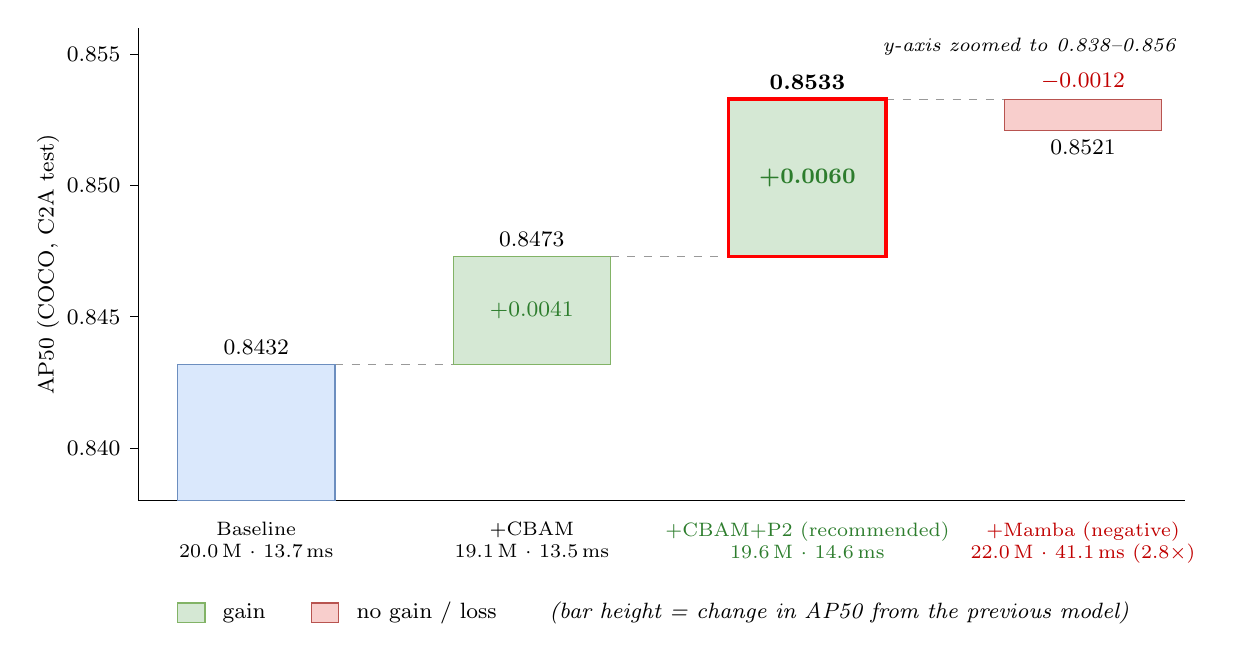
\begin{tikzpicture}[font=\footnotesize]
  % ---- axes ----
  \draw[black] (1.0,0) -- (1.0,6.0);
  \draw[black] (1.0,0) -- (14.3,0);
  \foreach \y/\lab in {0.6667/0.840, 2.3333/0.845, 4.0/0.850, 5.6667/0.855}{%
    \draw[black] (0.9,\y) -- (1.0,\y);
    \node[left] at (0.9,\y) {\lab};
  }
  \node[rotate=90,anchor=south] at (0.12,3.0) {AP50 (COCO, C2A test)};
  \node[anchor=north east,font=\itshape\scriptsize] at (14.3,6.0) {y-axis zoomed to 0.838--0.856};

  % ---- dashed step connectors ----
  \draw[wfGrey,dashed] (3.5,1.7333) -- (5.0,1.7333);
  \draw[wfGrey,dashed] (7.0,3.1)    -- (8.5,3.1);
  \draw[wfGrey,dashed] (10.5,5.1)   -- (12.0,5.1);

  % ---- bars ----
  \filldraw[fill=wfBaseFill,draw=wfBaseStroke]                     (1.5,0)      rectangle (3.5,1.7333);
  \filldraw[fill=wfGainFill,draw=wfGainStroke]                     (5.0,1.7333) rectangle (7.0,3.1);
  \filldraw[fill=wfGainFill,draw=wfRedEdge,line width=1.2pt]       (8.5,3.1)    rectangle (10.5,5.1);
  \filldraw[fill=wfMambaFill,draw=wfMambaStroke]                   (12.0,4.7)   rectangle (14.0,5.1);

  % ---- resulting AP50 above/below each bar ----
  \node[above] at (2.5,1.7333) {0.8432};
  \node[above] at (6.0,3.1)    {0.8473};
  \node[above,font=\footnotesize\bfseries] at (9.5,5.1) {0.8533};
  \node[below] at (13.0,4.7)   {0.8521};

  % ---- per-step delta ----
  \node[text=wfGreenText]                       at (6.0,2.4167) {+0.0041};
  \node[text=wfGreenText,font=\footnotesize\bfseries] at (9.5,4.1) {+0.0060};
  \node[above,text=wfRedText]                   at (13.0,5.1)   {$-0.0012$};

  % ---- x-axis labels: model, params, latency ----
  \node[below,align=center,font=\scriptsize] at (2.5,-0.15)
        {Baseline\\20.0\,M $\cdot$ 13.7\,ms};
  \node[below,align=center,font=\scriptsize] at (6.0,-0.15)
        {+CBAM\\19.1\,M $\cdot$ 13.5\,ms};
  \node[below,align=center,font=\scriptsize,text=wfGreenText] at (9.5,-0.15)
        {+CBAM+P2 (recommended)\\19.6\,M $\cdot$ 14.6\,ms};
  \node[below,align=center,font=\scriptsize,text=wfRedText] at (13.0,-0.15)
        {+Mamba (negative)\\22.0\,M $\cdot$ 41.1\,ms (2.8$\times$)};

  % ---- legend ----
  \filldraw[fill=wfGainFill,draw=wfGainStroke]  (1.5,-1.55) rectangle (1.85,-1.30);
  \node[anchor=west] at (1.95,-1.425) {gain};
  \filldraw[fill=wfMambaFill,draw=wfMambaStroke] (3.2,-1.55) rectangle (3.55,-1.30);
  \node[anchor=west] at (3.65,-1.425) {no gain / loss};
  \node[anchor=west,font=\footnotesize\itshape] at (6.1,-1.425) {(bar height = change in AP50 from the previous model)};
\end{tikzpicture}
